% Paper for Learning-Based Controls (ME 537)

\documentclass[letterpaper, 10 pt, conference]{ieeeconf}  % Comment this line out if you need a4paper

\IEEEoverridecommandlockouts                              % This command is only needed if 
                                                          % you want to use the \thanks command

\overrideIEEEmargins                                      % Needed to meet printer requirements.

\usepackage{prg-stuff}

\usepackage{caption}
\usepackage{subcaption}
\usepackage{algorithm}
\usepackage[noend]{algpseudocode}

\makeatletter
\def\BState{\State\hskip-\ALG@thistlm}
\makeatother

%\usepackage{ijcai09}  % style
\usepackage{times}    % font
\usepackage{graphicx} % inserting images
\usepackage{cite}
\usepackage{amsmath}
\usepackage{mathtools} % For math
\usepackage{hyperref}
\usepackage{float}
%\usepackage{enumitem}
\renewcommand{\deg}{\ensuremath{^{\circ}}\xspace}  % why doesn't this work???

\providecommand{\e}[1]{\ensuremath{\times 10^{#1}}}

\graphicspath{ {./figures/} } % Point to the figures directory

%%%%%%%%%%%%%%%%%%%%%%%%%%%%%%%%%%%%%%%%%%%%%%%%%%%%%%%%%%%%%%%%%%%%%%%%%%%

\title{\LARGE \bf 
Active Planning for Defect Detection in the Knife Domain
}

\author{Austin Nicolai, Kory Kraft, and Gabriel Hackebeil}

\begin{document}

\maketitle
\thispagestyle{empty}
\pagestyle{empty}

\begin{abstract}
\textit{Abstract text will go here}
\let\thefootnote\relax\footnote{\hrulefill
\\\hspace*{1em} \hfill
\\\hspace*{1em} Austin Nicolai and Kory Kraft
\\\hspace*{1em} Robotics Program, School of Mechanical, Industrial, and Manufacturing
\\\hspace*{1em} Engineering, Oregon State University, Corvallis, OR 97331, email: 
\\\hspace*{1em} {\tt\small \{nicolaia, kraftko\}@onid.oregonstate.edu}
\\\hspace*{1em} \hfill
\\\hspace*{1em} Gabriel Hackebeil
\\\hspace*{1em} Computer Science Department, School of Electrical Engineering and
\\\hspace*{1em} Computer Science, Oregon State University, Corvallis, OR 97331, email: 
\\\hspace*{1em} {\tt\small hackebeg@onid.oregonstate.edu}
}
\end{abstract}


\section{Introduction}


Defect detection is an interesting problem in automated manufacturing. Even though automated processes can be more consistent than human laborers, defects can occur due to a number of complex internal or external factors.  These defects can range from slight cosmetic blemishes to safety-threatening faults. The ability to quickly and accurately identify defects as soon as possible within the manufacturing process is important to ensure smooth operation, resource efficiency, and quality products.

Despite the advanced automated techniques used to manufacture complex products, many products are still manually inspected. This can cost companies and workers valuable resources.

With this in mind, this paper examines the above problems in the knife domain. The contributions of this paper are twofold:\\

\begin{enumerate}
	\item[1.] We analyze the effectiveness of using computer vision techniques with both adaptive planning and human-informed planning for active classification.\\
	\item[2.] We apply and test our approach to active classification in the knife domain with real-world data.\\
\end{enumerate}

\section{Related Work}

\subsection{Defect Detection}
Defect detection is necessary to ensure both quality and safety. The process of manually inspecting parts is tedious and error prone. Furthermore, it can be highly mentally and ergonomically redundant, decreasing employee satisfaction and leading to increased physical strain. Due to resource constraints within companies, it can sap skilled workers away from productive tasks, leading to economic losses.


Attempts and successes have been made in automating defect detection, but each defect detection process can be highly dependent upon the good manufactured \cite{defectGabor}\cite{defectSewer}. We have decided to focus on defects found during knife manufacturing. One example of this process involves quality assurance workers visually inspecting batches of knives for a wide variety of defects. Characterization of a defect varies between knife type, defect type, and defect severity. On average, a worker may spend four seconds (two per side) inspecting each knife and typically achieves an accuracy upper-bounded by 80\%.

\subsection{Computer Vision}

Computer vision, the automated extraction of meaningful information from images, relies on two key components for success: feature extraction and image classification. 

Feature extraction is necessary to deal with the extremely large datasets that comprise a single image.  For example, a small 64x64 RGB icon has 4096 individual pixels, each of which can be thought of as a unique feature. When looked at as a more complex feature composed of multiple pixels (i.e. the pixels that make up a nose verus an eye), the number of possible features is exponential. 


Feature extraction allows one to cut down the number of features examined from all possible features to a smaller, transformed subset of features that yields the most pertinent information. Feature extraction is different from feature selection in that feature selection simply grabs some subset of the original features and utilizes those \cite{featSelExt}.

While there are general methods currently in use across machine learning to deal with feature extraction (e.g. Principal Component Analysis) and selection, there are specific methods used in computer vision that take advantage of the image data structure.

Image classification is done using common machine learning techniques for classification. Machine learning comes in two forms: supervised and unsupervised. Unsupervised image classification is done by feeding an algorithm a large data set of images or videos and then allowing the machine to pick out the important features and classify these images. While still in its infancy, deep learning with neural networks has been used successfully. The problem with these algorithms at this stage is that they rely on extremely large data sets, can take a long time to train and run, and are not yet ready for a real-time vision system \cite{deepLearning1}. 

Unsupervised learning with image classification requires an expert to label a set of images beforehand. The labeled images are then used to instruct or train the classifier. While more tedious, given a large enough training set, these algorithms can be very efficient and effective.

For example, a real-time vision system for surface defect detection in steel manufacturing was successfully implemented by Jia, et al using standard supervised learning algorithms and a clever feature extraction scheme \cite{steelDefect}. The authors used a rough filter to detect possible edges in the steel and then features are extracted from that according to their pixel length, the gray scale constract of seam to adjacent area, the intensity differences between the two sides of the seams, and the mean and variance of the seam regions. Using these features, the images were then classified using two standard classification algorithms: K-Nearest Neighbors (KNN) and a Support Vector Machine (SVM). The authors were able to classify the images with greater than 90 percent accuracy at a rate of 172 images per second, fast enough to detect defects in real-time for a steel rolling machine that could reach speeds of 225 MPH.

A wavelet filter, Gabor filter, and Gabor wavlet filter were successfully used to classify corrugation defects on rail tracks\cite{railDefect}. In particular, the authors found the Gabor filter to be most successful. The image was first convolved with the Gabor filter at four different orientations. Each of these images were then evaluated with an energy distribution function yielding the mean and variance.  The mean and variance from each filter orientation were assembled to create a feature vector of size 8 for the original image. This is the filter we will be adapting for our approach.

\subsection{Adaptive View Planning}

Informative Path Planning (IPP) is defined as autonomously deciding what path to take while collecting measurements, based on a probabilistic model of the quantity being studied \cite{BNBIPP}. IPP has been effectively used to monitor environmental conditions with autonomous underwater vehicles\cite{BNBIPP}\cite{underwaterIPP}. IPP algorithms, when used in domains that exhibit the property of submodularity (e.g. sensor placement), yield simple greedy solutions that carry the important theoretical guarantee of a close approximation to the optimal solution (within ~63\% of optimal). Additionally, it can be seen that in many cases, greedy solutions are able to perform within 1\% of optimal. 

Adaptive View Planning (AVP) is a specialized case of IPP. AVP seeks to optimize the classification success rate in the shortest amount of time or lowest path cost by having an autonomous agent decide which view angles give the most pertinent information necessary to correctly classify a specific object. The planning is adaptive in the sense that what is seen from one view angle impacts which view angle the agent decide to move to and look at next\cite{hollinger2011active}. 

This problem has been examined in the domain of examining ship hulls for mines \cite{hollinger2011active}. The authors reduced the number of needed views by 80 percent compared to non-adaptive methods.

\section{Methods}

\subsection{Data Generation}

In order to accurately detect surface defects in knives, a classifier must be trained. To ensure the classifier is robust, it must be trained on a large, and comprehensive, set of data.

In generating our data, the knives were first filmed under a variety of lighting conditions from multiple angles. Still images were then extracted to create a training set. The images selected represent many different angles and several lighting conditions. In the image set, there exist both positive and negative examples of the defect.

Next, a sliding window technique was used to generate additional training data from the image set. This process is shown in \textit{Figure \ref{fig:data generation}}. This was accomplished using a custom program that allows a user to specify the location of all defect corners. From this, the sliding window is able to automatically determine if the region contains a defect. Using this information, the program is able to automatically label the training set data for use in supervised learning.

\begin{figure*}
    \centering
    \begin{subfigure}[b]{.32\textwidth}
        \centering
        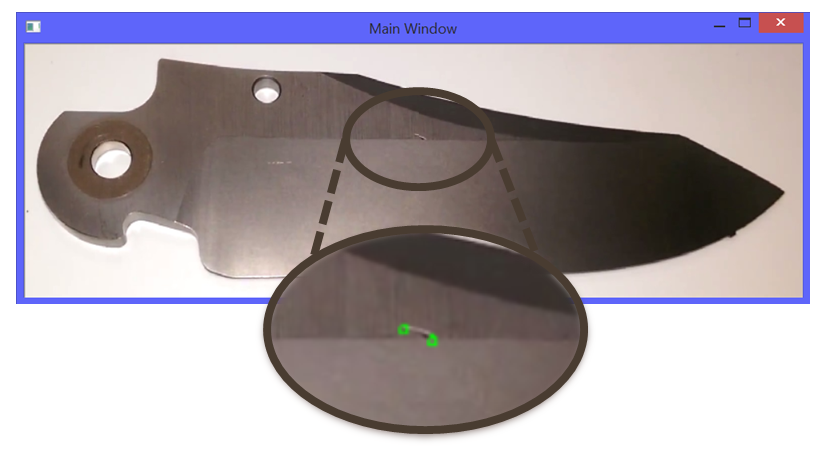
\includegraphics[width=.9\textwidth]{defect_location.png}
        \caption{Selected defect corners}
        \vspace*{2mm}
        \label{fig:defect corners}
    \end{subfigure}
    \hfill
    \begin{subfigure}[b]{.32\textwidth}
        \centering
        \raisebox{8.2mm}
        {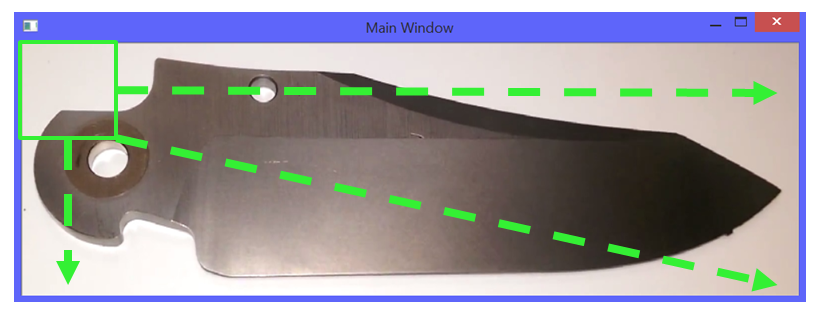
\includegraphics[width=.9\textwidth]{defect_sliding_window.png}}
        \caption{Sliding window}
        \vspace*{2mm}
        \label{fig:sliding window}
    \end{subfigure}
    \hfill
    \begin{subfigure}[b]{.32\textwidth}
        \centering
        \raisebox{1.7mm}
        {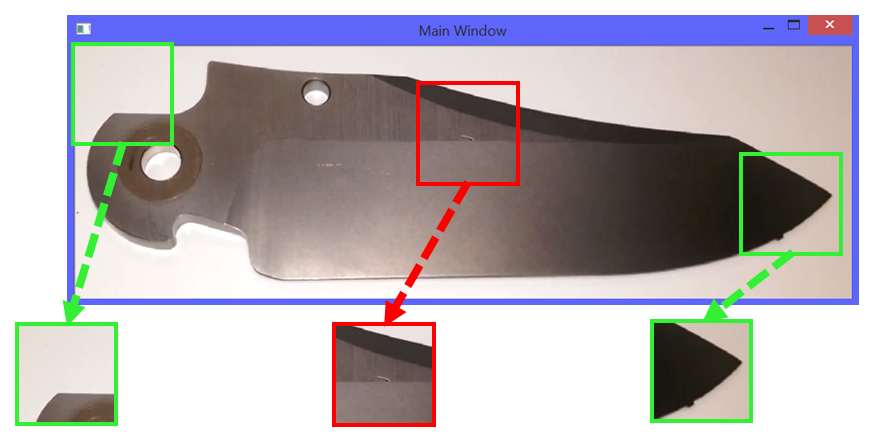
\includegraphics[width=.9\textwidth]{defect_windows.png}}
        \caption{Example labeled windows}
        \vspace*{2mm}
        \label{fig:labeled windows}
    \end{subfigure}
    \caption{Training data generation}
    \label{fig:data generation}
\end{figure*}

\subsection{Computer Vision Algorithm}

The computer vision algorithm employed in this paper was first proposed by for use in defect detection in railroad tracks \cite{railDefect}. The algorithm uses Gabor filters and an energy distribution function to extract features from an input image. The classification is performed by an SVM classifier. A flowchart of the algorithm can be seen in \textit{Figure \ref{fig:vision algorithm diagram}}.

First, the input image is fed through a filter bank consisting of Gabor filters. Four wavelet orientations are used: \textit{0\degree}, \textit{45\degree}, \textit{90\degree}, and \textit{135\degree}. Each orientation is replicated for three different filter sizes. This yields a total of twelve filters. Next, the magnitude operator is applied to the filtered images. 

The next step is feature extraction for input into the SVM. The features used are the mean and variance of each filtered image. This allows for an image of high resolution to be collapsed down into a manageable feature set. The final resulting feature vector consists of all means and variances. For our algorithm, the feature vector is of length 24. An example of the entire process can be seen in \textit{Figure \ref{fig:gabor filter bank}}.

\begin{figure*}
    \centering
    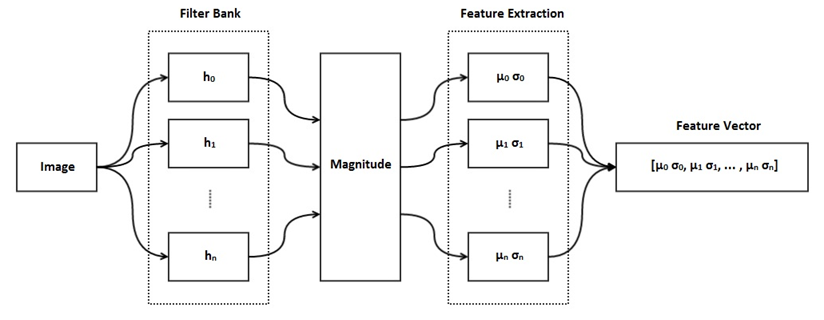
\includegraphics[width=.75\textwidth]{computer_vision_diagram.png}
    \caption{Computer vision algorithm flowchart}
    \vspace*{2mm}
    \label{fig:vision algorithm diagram}
\end{figure*}

\begin{figure}
    \centering
    \begin{subfigure}[b]{.49\textwidth}
        \centering
        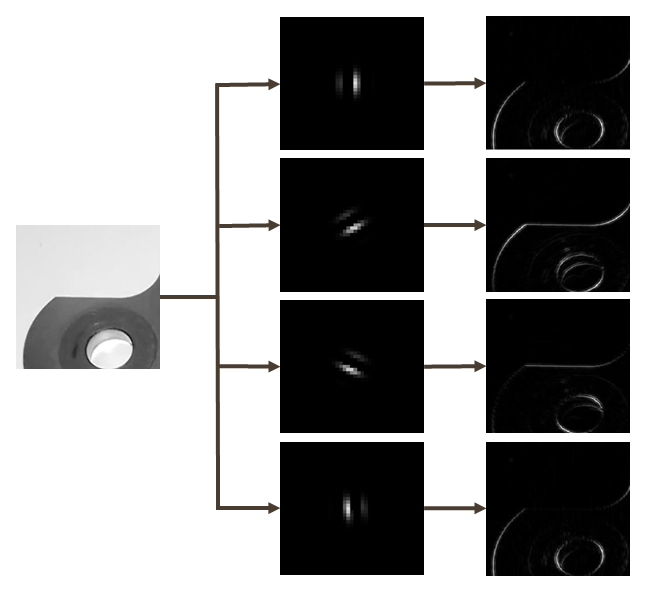
\includegraphics[width=.65\textwidth]{gabor_filter_small.png}
        \caption{Small Gabor filter bank}
        \vspace*{2mm}
        \label{fig:small gabor}
    \end{subfigure}
    \hfill
    \begin{subfigure}[b]{.49\textwidth}
        \centering
        {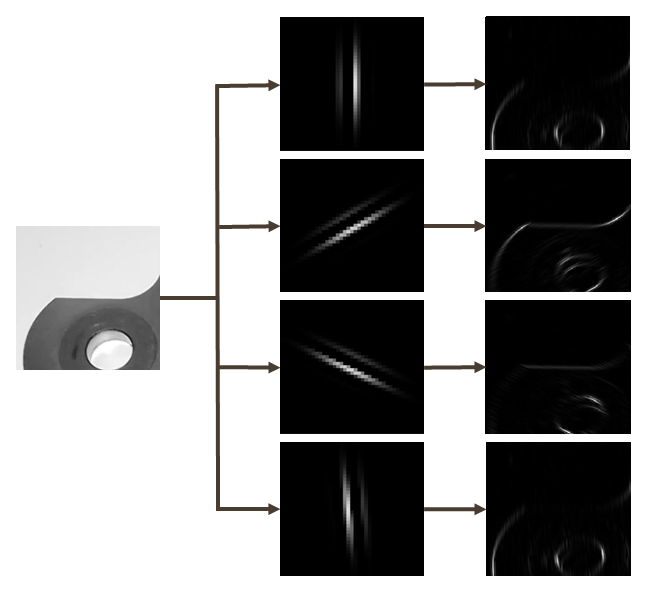
\includegraphics[width=.65\textwidth]{gabor_filter_large.png}}
        \caption{Large Gabor filter bank}
        \vspace*{2mm}
        \label{fig:large gabor}
    \end{subfigure}
    \caption{Gabor filter bank examples}
    \label{fig:gabor filter bank}
\end{figure}

\subsection{Adaptive Planning}

We propose to incorporate an informative path planning approach to maximize detection of potential knife defects. Informally, such a procedure will require training against a sufficiently large image database so that knife regions can be identified as showing potential for having a surface defect.

Such a path planning problem seems trivial until placing strict timing constraints on the image capturing procedure or as we limit the number preset camera locations. Given a single fixed camera location, we assume a robot arm (e.g. a Motoman Education Cell) is available for grasping a single knife and rotating it to the appropriate angle for the camera to capture a specific view. Additionally, changes to the lighting configuration, or lighting type (e.g. near field, dark field), could be used to specify a different view configuration.

Initially, we assign equal information to all locations along the knife surface. Naturally this leads to the first view capturing one full side of the knife edge. Subsequent views will be based on the information yielded during image analysis. Potential defect locations identified by the analysis will lead to an updated non-uniform information layout along the knife surface. High probability of defect detection on one location of the knife might lead to the next view being zoomed in near that knife region. If the image analysis does not lead to significant potential defect locations, the original information layout would likely cause the path planning algorithm to capture a full view of the information on the opposite knife edge.

The order in which views will be selected by the planner will depend upon the predicted information gain. This will be calculated by the standard method of entropy reduction. That is, the selected view will be the one in which the resulting defect probability distribution will be most certain. One of the challenges in this approach lies in predicting the results of viewing a specific view. This, in part, can be achieved through using the expected output of the vision system. This is one reason why it is important for the vision system to be robust.

Additional considerations such as reflection angle against light resources could have a significant effect on how well knife defects are identified in images will need to be considered. In most cases, the physical manifold changes between knife types. Given the knife surfaces particular to the current knife unit being examined, a single image capture could be replaced with multiple image captures at different reflection angles to maximize the possibility of defect discovery.

\subsection{Human-Informed Planning}

In addition to adaptive planning, we will investigate the use of incorporating actual human inspection paths in the path planning algorithm. The motivation for this is that through experience, skilled human inspectors build a large knowledge base of how/where defects typically present. This allows them to inspect knives more effectively than a novice. We theorize that in most cases, human inspectors will follow a general view sequence that they have learned works well. When the inspector notices something that is a potential defect, they may adjust their view sequence to more closely inspect that area.

This data can be incorporated into the adaptive view planning algorithm by using it to help adjust information levels along the knife surface. That is, if a human inspector typically transitions from one view to small subset of views, we can inflate the information in regions that will increase the likelihood of the planner to select that subset of views.

Additionally, with information on when in their view sequence the inspectors believe they see defects, we can more accurately adjust the region information values. For example, inspectors may generally transition from their current view to a given subset of views. However, if they believe they see a defect, perhaps they will iterate through a different subset of views to further inspect the current region. We can use this information to adjust which regions of information we inflate based upon the actual, or expected, output of the vision system. That is, if the vision system strongly believes a defect to be present in a region, we may inflate the information values of one subset of regions. However, if the vision system believes a region to be clear of defects, we may inflate a different subset of regions.

\section{Results}

\subsection{Computer Vision Algorithm}

Initial testing of the proposed vision algorithm shows good results. Initial results show that for training, validation, and test data sets, the defect detection rate is greater than 80\%. It is important to note that while promising, these results were generated from a limited data set in terms of knife and defect examples. Increasing the number of examples, both positive and negative, in the data set will yield a more robust classifier.

While additional parameter tuning in the vision algorithm may yield higher detection rate, there are other avenues to explore. These avenues include the use of alternative lighting sources (e.g. near field, dark field), as previously mentioned. The use of these lighting sources may help to increase the visibility of defects, and thus make them easier to classify. This, in turn, will lead to a higher defect detection rate for the classifier.

\subsection{Adaptive Planning}

\textit{Adaptive Planning results text will go here}

\subsection{Human-Informed Planning}

\textit{Human-Informed Planning results text will go here}

\section{Discussion}

\textit{Discussion text will go here}

\section{Conclusions and Future Work}

\textit{Conclusions and Future Work text will go here}

\bibliographystyle{IEEEtran}
\bibliography{main}


\end{document}

% FIGURE HINTS 
%
%\begin{figure*}
%    \centering
%    \begin{subfigure}[b]{0.3\textwidth}
%        \centering
%        \includegraphics[width=.7\textwidth]{Reflex.jpg}
%        \caption{Reflex agent path}
%        \label{fig:reflex path}
%    \end{subfigure}
%    \hfill
%    \begin{subfigure}[b]{0.3\textwidth}
%        \centering
%        \includegraphics[width=.7\textwidth]{Random.jpg}
%        \caption{Random agent path}
%        \label{fig:random path}
%    \end{subfigure}
%    \hfill
%    \begin{subfigure}[b]{0.3\textwidth}
%        \centering
%        \includegraphics[width=.7\textwidth]{Memory.jpg}
%        \caption{Memory agent path}
%        \label{fig:memory path}
%    \end{subfigure}
%    \caption{Agent paths}
%    \label{fig:agent paths}
%\end{figure*}

% ALGORITHM HINTS
%
%\begin{algorithm}[h]
%\caption{Reflex agent}\label{reflex algorithm}
%\begin{algorithmic}[1]
%\If {$isDirty = true$}
%\State \Return \textit{actionSuck}
%\ElsIf {$facingWall \neq true$}
%\State \Return \textit{actionForward}
%\ElsIf {$facingWall = true$ AND $isHome = true$}
%\State \Return \textit{actionOff}
%\Else
%\State \Return \textit{actionTurnRight}
%\EndIf
%\end{algorithmic}
%\end{algorithm}
